\setchapterpreamble[u]{%
\dictum[Douglas Adams]{A common mistake that people make when trying to design something completely foolproof is to underestimate the ingenuity of complete fools. \dots}}
\chapter{System- und Softwareentwurf} \index{System- und Softwareentwurf}\label{kap:systemundsoftwarentwurf}


Dieses Kapitel beschreibt den System- und Softwareentwurf sowie die Auswahl der Umgebung, Plattform, Software, Programmiersprache und Frameworks.

\section{Auswahlprozess}

Teil der Aufgabe der Arbeit ist es, für das System im Rahmen der nichtfunktionalen Anforderungen eine geeignete Laufzeitumgebung zu schaffen. Dafür sind einige Entscheidungen zu treffen. 

\subsection{Webservice}\index{Webservice}\label{sec:webservice}
Wenn von Webservices gesprochen wird, dann werden meistens \gls{SOAP}-basierte Webservices gemeint. Allerdings gibt es die sogenannten \gls{SOAP}-basierten Webservices als auch die \gls{REST}ful Webservices. Anforderung ist es ein Web Service zu implementieren. Dazu muss entschieden werden, ob ein \gls{SOAP}-basierter oder \gls{REST}ful Webservice implementiert werden soll. \index{REST@\textbf{REST}} \index{REST!RESTful}

\subsubsection{Definition}

\begin{quotation}
\enquote{Web services provide the means to integrate disparate systems and expose reusable business functions over HTTP. They either leverage HTTP as a simple transport over which data is carried (e.g., SOAP/\gls{WSDL} services) or use it as a complete application protocol that defines the semantics for service behavior (e.g. RESTful services) \citep[S. 2][]{robinsonService}}	
\end{quotation}

\subsubsection{SOAP/WSDL Webservice}\index{SOAP}\index{WSDL}\index{Webservice}
Frau Janssen hat in ihrer Abschlussarbeit einen Webservice nach ISO 29002-20 mittels einem SOAP/WSDL Webservice implementiert \citep[vgl.][]{janssen}. Die ISO 29002-20 verweist in Annex-B auf entsprechende WSDL-Definitionen. 
Ich möchte an dieser Stelle darauf verzichten, die Einzelheiten eines SOAP/WSDL Webservice zu erläutern und verweise auf Frau Janßens Abschlussarbeit \citep[vgl.][Kap. 3]{janssen}. 

Es sei an dieser Stelle kurz erwähnt, dass Webservices auf SOAP/WSDL basierend ein W3C\footnote{World Wide Web Consortium - http://www.w3.org} Standard sind. Dies ist häufig auch ein Kriterium, weshalb in der Industrie \gls{SOAP}/WSDL \glspl{Webservice} stark verbreitet sind. 

\subsubsection{RESTful Webservice}\index{RESTful Webservice}\index{REST@\textbf{REST}} \index{REST!RESTful} \index{REST!RESTful Webservice}
\gls{REST}ful Webservices sind per se kein Standard sondern eher ein Programmierparadigma respektive ein Architekturmuster. 
Stefan Tilkov schreibt dazu in seinem Buch \enquote{Rest und HTTP: Einsatz der Architektur des Web für Integrationsszenarien} \citep[S.10][]{tilkovrest}, folgendes:

\begin{quotation}
\enquote{...Im Rahmen seiner Dissertation - beendet im Jahre 2000 - abstrahierte Fielding\footnote{Anmerkung des Autors: Roy Thomas Fielding} von der konkreten Architektur, die HTTP zugrunde liegt, und legte den Schwerpunkt auf die Konzepte anstatt auf die konkrete Syntax, die Details des Protokolldesigns und die vielen Kompromisse, die aus Kompatibilitätsgründen eingegangen werden mussten. Als Ergebnis entstand der Architekturstil REST. Dieser ist somit eine Stufe abstrakter als die HTTP-Architektur: Theoretisch könnte man die Prinzipien von REST auch mit einem neu erfundenen Satz von Protokollen umsetzen. In der Praxis ist jedoch tatsächlich nur das Web als konkrete Ausprägung des Architekturstils relevant...}
\end{quotation}
\citep[Vgl. auch][]{fieldingrest}

\subsubsection{Fazit}
Die Analyse aus \autoref{kap:analyse_und_definition} zeigt, dass eine Abfrage (Query) gemäß Standard als XML dargestellt wird. Diese XML-Dateien müssen folglich an das System gesendet werden. Demnach ist eine Lösung mittels \gls{SOAP} \gls{Webservice} als auch \gls{REST}ful \gls{Webservice} denkbar. 
Es wurde ein \gls{REST}ful \gls{Webservice} ausgewählt. Die Gründe stellen sich wie folgt dar:

\begin{description}
\item[Einfache Implementierung] Da \gls{REST}ful Webservices auf dem HTTP Protokoll basieren und ferner sehr gute und geeignete Frameworks für Java vorhanden sind, siehe \autoref{kap:bibliotheken_und_frameworks}, stellt sich für Web Entwickler die Implementierung als einfach heraus. \gls{SOAP} \glspl{Webservice} sind per se etwas komplexer, da \gls{SOAP} ein eigenes Protokoll darstellt. 
\item[Payload XML] Der Payload des Anfrage-Queries wird als XML angegeben (siehe \autoref{fig:datenfluesse}. Als mögliche Übertragung wird email angegeben. Für die Anforderungen dieser Arbeit bedeutet dies eine Implementierung eines \glspl{Webservice}, welcher die XML-Repräsentation des Queries als Payload mittels XML überträgt. Folglich könnte sowohl \gls{SOAP} als auch \gls{REST} benutzt werden. Voraussetzung ist eine definierten Schnittstelle, welche lediglich ein XML als Payload akzeptiert. 
\item[Kein Vorteil bei SOAP] Somit hat \gls{SOAP} keinen Vorteil gegenüber \gls{REST}. Der Vorteil würde darin bestehen, wenn \gls{SOAP} selbst die Operationen anbietet (definiert in der \gls{WSDL}). Das hat den Nachteil, dass die wohlgeformte vorgegebenen Schemata query.xsd, in der Form nicht genutzt werden können. Es muss somit eine Einbindung in \gls{SOAP} erfolgen.
 \item[Vorteil des Payloads] Der klare Vorteil bei der Variante eine Query XML-Datei gemäß query.xsd Schema des Standards als Payload zu versenden ist der, dass eine Validierungsprüfung der XML gegen vorhandene definierte Regeln des Schemas erfolgen kann (z.B. gültige \gls{IRDI}), ferner können aus dem Schema passende Modellklassen zur Verarbeitung und Speicherung der Query-Daten in der Applikation generiert werden. Mehr Informationen gibt es in \autoref{sec:modellgenerierung}. 
\item[SOAP Webservice bereits im Einsatz] Ein weiterer Grund ist der, dass Frau Janßen in Ihrer Abschlussarbeit bereits einen SOAP-Webservice einsetzt. Nennen wir es Vielfältigkeit der Technologien im Fachbereich, jedenfalls bietet es die Möglichkeit eine weitere Technologie zu betrachten, einzusetzen und ggfs. zu vergleichen. 
\end{description}

\subsection{Plattform} \index{Apache Tomcat} \label{sec:plattform}
Als Laufzeitumgebung kann prinzipiell ein beliebieger Web Container bzw. Web Server ausgewählt werden, welcher Webservices, sei es \gls{REST}ful \glspl{Webservice} oder \gls{SOAP} \glspl{Webservice}, unterstützt. 
Es wurde der \gls{Apache Tomcat} Server in der Version 7 ausgewählt. Das ist ein üblicher Web Container (Web Server), welcher mit entsprechenden Frameworks bzw. Bibliotheken sowohl \gls{SOAP} als auch \gls{REST}ful \glspl{Webservice} anbieten kann. 

Folgende Server sind zum Einsatz ebenfalls möglich:

\begin{description}
\item[Jetty] http://www.eclipse.org/jetty/
\item[Tomcat] https://tomcat.apache.org/
\item[JBoss] https://www.jboss.org/overview/
\end{description}

Festzuhalten sei noch, dass es sich beim JBoss Server um einen sogenannten Application Server handelt. Er verfügt zusätzlich über eine Web Container Funktionalität noch über weitere Dienste, wie beispielsweise Transaktionsmanagement, Security oder verteilte Applikationsunterstützung. 

\subsection{Bibilotheken und Frameworks} \index{Bibilotheken und Frameworks}\label{bibliotheken_und_frameworks}
\begin{description}

\item[Jersey] Framework zur Erstellung von RESTful Web Services \index{Jersey}\gls{Jersey}
\item[JSF2.0] Komponentenbasiertes Web Framework zur Erstellung von Benutzeroberflächen \index{JSF2.0}
\item[Spring] Dependency Injection Framework. Bietet darüber hinaus noch weitere Komponenten an. Ausgewählt wurde unter anderem \gls{Spring} JDBC und \gls{Spring} Data Oracle, welche einfacheren Zugriff auf relationale Datenbanken sowie auf Prozeduren von relationalen Datenbanken ermöglicht. Mehr Details zur Implementierung in Kapitel \todotext{Kapitel angeben}. \index{Spring} 
    
\end{description}

\todotext{Eine detaillierte Erklärung der Frameworks nötig, Erläuterung des Nutzens und weshalb diese ausgesucht wurden. Ggfs in Anhang}

\subsection{Programmiersprache}
Vorgegeben ist die Umsetzung eines \glspl{Webservice}. Diese lassen sich in fast allen aktuellen Programmiersprachen entwickeln, folglich kann prinzipiell jede Sprache ausgewählt werden die Webservices anbieten kann.  

Es wurde die Sprache Java gewählt, da diese zum einen in der aktuellen Industrie stark verbreitet und zum anderen der Autor dieser Arbeit seit vielen Jahren damit vertraut ist. Ferner besteht hier eine Abhängigkeit zur Auswahl der Plattform gleichsam des Web Containers, siehe \autoref{sec:plattform}. Beim Einsatz von Java ist man an einen Web Container (Web Server) gebunden, welcher auch Java unterstützt. 

Ein weiterer Aspekt ist, dass Software welche mit Java entwickelt wurde im Prinzip auf jedem Betriebssystem lauffähig, und somit portierbar ist. Dies ist zwar keine Anforderung des Projektes, aber ermöglicht die Arbeit und Entwicklung in beliebigen Systemen. 

\section{Softwaredesign und Architektur}

\subsection{Bausteinsicht}\index{Software-Bausteine}
\begin{quotation}
Die Bausteinsicht bildet die Aufgaben des Systems auf Software-Bausteine oder -Komponenten ab.
 \citep[S. 98ff][]{starke}	
\end{quotation}

Es soll mit Hilfe dieser Sichten ein Überblick über den Aufbau des Systems und den Abhängigkeiten der einzelnen Komponenten geschaffen werden. Dazu wird das System im top-down Ansatz aufgezeigt und verfeinert. 

Die Kontextabgrenzung zeigt das System im Zusammenspiel mit anderen Systeme und zeigt somit gleichsam die Systemgrenzen auf. 

\subsubsection{Kontextabgrenzung - Systemüberblick und angrenzende Systeme} 

\begin{figure}[htbp]
	\centering
		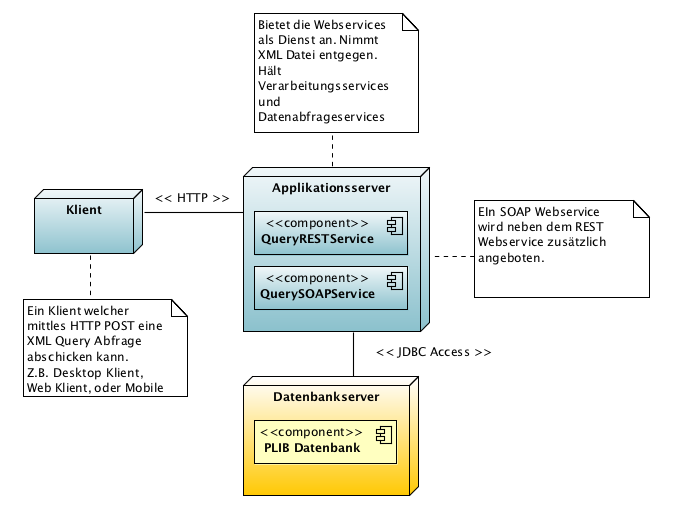
\includegraphics[width=0.9\textwidth]{images/bausteinsicht_plib_level0.png}
	\caption{Bausteinsicht - Kontextabgrenzung}
	\label{fig:bausteinsicht_level0}
\end{figure}

\paragraph{Klient}

Der Klient stellt den Nutzer des Query Services dar. Er erzeugt das XML File, welches als Query an den Service geschickt wird. Der Transport erfolgt über das HTTP Protokoll.  

\paragraph{Applikationsserver}

Der Applikationsserver ist der Hauptbaustein. Dieser Baustein enthält alle entwickelten Komponenten. Sichtbar von außen ist der QueryService, dieser Service ist ein REST WebService und nimmt XML-Dateien als Payload eines POST Requests entgegen. 

\paragraph{Datenbankserver}
Der Datenbankserver beinhaltet die PLIB Datenbank mit den entsprechenden Zugriffsprozeduren auf die Daten.

\subsubsection{Level 1 - Plib characteristic query} 

Die Bausteinsicht Level 1 zeigt alle Komponenten des entwickelten Systems auf und deutet die externen Schnittstellen an. Mittels <<use>> Beziehungen erkennt man die Abhängigkeiten der einzelnen Komponenten. 

\begin{figure}[htbp]
	\centering
		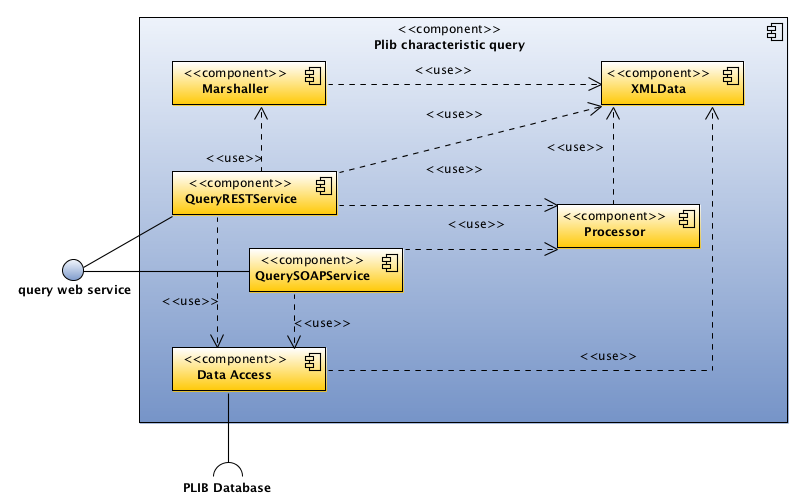
\includegraphics[width=0.98\textwidth]{images/bausteinsicht_plib_level1.png}
	\caption{Bausteinsicht - Level 1}
	\label{fig:bausteinsicht_level1}
\end{figure}

\begin{description}
\item[QueryService] Der Zweck dieser Komponente ist das Entgegennehmen des Requests (Query-XML File), das Weiterleiten an die weiterverarbeitenden Komponenten und letztlich das Zurücksenden der Rückantwort (Katalog-XML). Bietet nach Außen die \gls{Webservice}-Schnittstelle an.
\item[Data Access] Diese technische Komponente beinhaltet die Zugriffsschicht auf die externe Datenbankschnittstelle und bietet entsprechend vereinfachte Abfrageschnittstellen für die anderen Komponenten an. 
\item[Marshaller] Eine weitere technische Komponente, diese ist für das Einlesen und Validieren der eingegangenen Query-XML Datei verantwortlich. Ferner transformiert diese Komponente die Informationen aus der Query-XML nach Validierung in das im System benutze Datenmodell aus der Komponente XMLData.
\item[XMLData] Beinhaltet das Datenmodell des Systems. Sowohl die eingehenden Query-XML Daten, als auch die ausgehenden Katalog-XML Daten werden intern in ein entsprechendes Model zur Verarbeitung abgelegt, so dass darauf gearbeitet werden kann.  
\item[Analyser] Diese Komponente ist für die Analyse des Queries, welches bereits als Modell vorliegt, verantwortlich. Erkennt ob es sich um einen \enquote{Simple Query} oder um einen \enquote{Parametric Query} handelt und leitet den Query zur Weiterverarbeitung an die Handler-Komponente weiter. 
\item[Handler] Erhält den Query vom Analyser und verarbeitet gemäß der Erkennung vom Analyser den Query weiter. Dazu werden die Querydaten gemäß des Datenbankmodells transformiert und die Data Access Komponente aufgerufen. Die Antwort der Data Access Komponente wird in das entsprechende Modell für die Katalogdaten umgewandelt und zurück an den Handler geleitet.  
\end{description}

\subsubsection{Level 2 - Whiteboxansicht - Komponente XMLData} 

Die Komponente XMLData beinhaltet alle Datenmodelle für die beiden Hauptkonzepte \enquote{Query for characteristic data} nach. 

\begin{figure}[htbp]
	\centering
		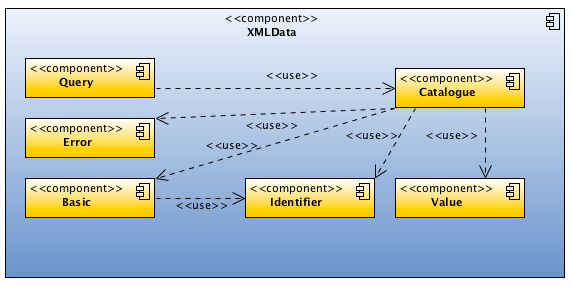
\includegraphics[width=0.82\textwidth]{images/bausteinsicht_plib_level2_xmldata.png}
	\caption{Bausteinsicht - Level 2 - Komponente XMLData}
	\label{fig:bausteinsicht_level2_xmldata}
\end{figure}

\begin{description}
\item[Query] Diese Komponente beinhaltet das Datenmodell des Queries nach ISO/TS 29002-31. 
\item[Catalogue] Diese Komponente beinhaltet das Datenmodell des Kataloges nach ISO/TS 29002-10. 
\item[Basic] Diese Komponente beinhaltet das Datenmodell von Basistypen nach ISO/TS 29002-4.
\item[Value] Diese Komponente beinhaltet das Datenmodell der Wertetypen nach ISO/TS 29002-10.
\item[Identifier] Diese Komponente beinhaltet das Datenmodell für Identifier (IRDI) nach ISO/TS 29002-5. 
\end{description}

\todotext{Whiteboxansicht der Komponente Handler und Analyser einfügen zum besseren Verständnisses, ggfs. alle detaillierten Whiteboxansichten in Anhang?!}
